\documentclass[main.tex]{subfiles}
\begin{document}
\onlyinsubfile{\mainmatter{}}

\chapter{Glyco: A Nanopass Compiler for CHERI-RISC-V}
Glyco\footnote{From the Greek term $\gamma\lambda\upsilon\kappa{}o$ meaning \enquote{sweet}, alluding to the taste of a wild cherry.} is a compiler targeting the CHERI-RISC-V architecture, producing software running on CheriBSD systems and on a Sail-based emulator of the CHERI-RISC-V ISA.

We begin by giving a concise description of the nanopass compiler design, which is used for Glyco. We then describe the design \& implementation of the base compiler, a compiler that emits CHERI-RISC-V instructions but has almost no additional features taking advantage of the capability machine proper. We do so using a few example programs, working our way from the high-end language to the machine language. A full language reference of the final compiler can be found in \cref{ch:grammar}.

Later chapters discuss extensions and changes to this first version of the compiler.

\section{Background: Nanopass Compilers}
Glyco is built following a \emph{nanopass} compiler design, described in the context of compiler education by several authors such as \cite{educomp} and in the context of commercial compiler development by authors such as \cite{commcomp}. A nanopass compiler consists of numerous small passes, so-called \emph{\glspl{nanopass}}, which translate one \emph{\il{}} to another. Source code is parsed into the compiler’s first \il{}, which is then translated via \glspl{nanopass} through different \ils{}, ending up in the compiler's final \il{}. This final \il{} contains a string representation of the assembly code that is fed to the Clang compiler from the LLVM compiler toolchain for building \& linking an executable ELF file. This last step is unrelated to the research problem, hence this dependency on LLVM.

The nanopass design allows the compiler engineer to design and implement their compiler \emph{by iterated abstraction}. A simplified description follows. The engineer first chooses a target language (usually a machine language such as x86-64 or indeed CHERI-RISC-V) and determines an abstraction over it. The engineer then defines an \il{} that implements that abstraction as well as a \gls{nanopass} which transforms programs written in the new \il{} to the target language. The compiler engineer then repeats this process, this time abstracting over the \il{} with a new \il{} and \gls{nanopass}. This process goes on until a level of abstraction has been reached that can either be directly used as a source language (by human users), or be easily produced by parser actions.

An important benefit of the nanopass approach is each new iteration begins and ends with a working compiler. After each iteration, users can start writing and compiling programs in the new \il{} and unit tests can be written that ensure that the new \gls{nanopass} produces the expected transformations. For experimental architectures such as CHERI-RISC-V, this also means that designers can experiment more quickly with new ideas, something that may be harder to do on a full-fledged production compiler such as Clang.

Glyco defines 20 \gs{il}. Each language is named after the new abstraction or feature it brings compared to the \g{lowerlang}. We discuss these \gs{il} in reverse chronological order (from high-level to low-level languages) as opposed to the order in which the \gs{il} were defined (from low-level to high-level languages). This allows us to explain the compiler pipeline using example programs, showing how they are manipulated by the compiler's \gs{nanopass}.

\section{An Expression Language}
The highest \il{} in the first version of Glyco is called \textbf{EX} (Expressions), a language with basic support for arithmetic operations, functions, conditionals (if-then-else), definitions (let-bindings), vectors (fixed-size arrays), and records (collections of key-value pairs).

The following EX program computes the 30th number in the Fibonacci sequence starting with 0 and 1:
\lstinputlisting{Programs/fib.ex}

This program defines a function \texttt{fib} with three signed 32-bit integer parameters \texttt{prev}, \texttt{curr}, and \texttt{iter} and which returns a signed 32-bit integer. The function recursively adds the \enquote{previous} and \enquote{current} sums until the number of iterations drops to 0, then returns the \enquote{current} sum. The program itself is defined as the result of \texttt{fib} where \texttt{prev} is 0, \texttt{curr} is 1, and \texttt{iter} is 30.

EX is an \emph{intermediate} language and not necessarily a \emph{user-friendly} language; it is instead quite explicit and contains little syntactical sugar. For example, a value representing the constant 30 is written as \texttt{constant(30)}, the value of a variable or parameter named \texttt{iter} is written as \texttt{named(iter)}, and the predicate $ \textit{iter} \le 0 $ is written as \texttt{relation(named(iter), le, constant(0))}. A significant benefit is that the structure is easy to manipulate as the code goes through the compiler's \gs{nanopass}. One can, however, define a more user-friendly language and write a parser that emits EX.

EX is \lowered{} to \textbf{LS} (Lexical Scopes). LS does not support subexpressions so the \g{nanopass} binds all subexpressions to names and uses those names in place of the subexpressions. Our Fibonacci example now becomes:
\lstinputlisting{Programs/fib.ls}

LS is itself \lowered{} to \textbf{DF} (Definitions) which does not support shadowing. For instance, the following LS program defines \texttt{answer} twice but only uses the outer definition. Without shadowing, the program would evaluate to 28. The right answer is 42.
\lstinputlisting{Programs/shadowing.ls}

The \g{nanopass} to DF implements shadowing by renaming symbols such that each definition uses a globally unique symbol.
\lstinputlisting{Programs/shadowing.df}

Definitions in value position in DF are implemented using \enquote{computed values} (\texttt{do} values) in \textbf{CV} (Computed Values), which are values on which a computation can be attached. The previous DF program is \lowered{} to the following CV program without definitions, i.e., without let-bindings, and with \texttt{do} values instead:
\lstinputlisting{Programs/shadowing.cv}

Computed (\texttt{do}) values are themselves implemented by flattening them and binding the result to a name. The \g{nanopass} produces a \textbf{CA} (Canonical Assignments) program. The previous CV program becomes the following CA program, in which it becomes even clearer that the defined symbol with value 28 is not used anywhere in the program:
\lstinputlisting{Programs/shadowing.ca}

A \enquote{value}, in programming language parlance, is a placeholder for a datum at runtime. In Glyco, a value is an abstraction that is introduced in CA and expanded in the aforementioned higher \gs{il}. They represent the result of one of the effects that are available in its \g{lowerlang}, \textbf{CC} (Calling Convention). For instance, the CA program
\lstinputlisting{Programs/values.ca}
is \lowered{} as the following CC program:
\lstinputlisting{Programs/values.cc}

\section{A Conventional Calling Convention}
A \g{cc} is a set of rules imposed by the operating system, instruction set architecture, and/or programming language that specify how procedures are called. A low-level \g{cc} often specifies
\begin{itemize}[noitemsep]
	\item where parameters and result values are placed (in dedicated registers, in a particular order on the call stack, or a combination of both);
	\item how large values are passed to the callee or caller (over multiple registers, on the call stack, or in heap memory);
	\item the state of the call stack and some registers (like the register keeping the frame pointer) when a procedure starts executing or when it returns to the caller;
	\item which registers a procedure can use freely but for which it cannot assume that their contents will be preserved across a procedure call (\gs{cersaved}); and
	\item which registers a procedure can only use after saving their previous contents and if they're restored after use (\gs{ceesaved}).
\end{itemize}

The \g{cc} used in base version of Glyco is called \textbf{\g{ghscc}} and mimics a traditional \g{cc} that would be used for programs written in C, with some parts specified by \cite[chapter~25]{riscv}.

\paragraph{Call Stack} The call stack is a region of memory on which information about procedure calls is stored, such as local state and return addresses. The stack grows downward, i.e., from high to low addresses. The \texttt{csp} register contains a capability, the \textbf{\g{stackcap}}, that points to the location of the last pushed datum, i.e., the top of the stack. The \g{stackcap}'s address decreases whenever data are pushed to the call stack and increases whenever data are popped from the stack.

\paragraph{Call Frames} A call frame (also known as a \emph{stack frame}) is a region of memory on the call stack that belongs to a procedure call and on which the procedure can store its local state. The \texttt{cfp} register contains a capability, the \textbf{\g{framecap}}, that points to the base of the call frame. The procedure places local state and expects parameters in locations that are fixed distances removed from this base.

Before accessing its call frame, a procedure pushes a call frame of the desired size in three steps. The procedure first pushes the (caller's) \g{framecap} to the call stack, then updates the \g{framecap} to point to this capability, and finally allocates room for its local state by moving the \g{stackcap} so that it points to the call frame's last datum.

A procedure pops its call frame when it is done using it, e.g., when returning to its caller. It does so by popping all data stored in the call frame and restoring the previous \g{framecap}.

% TODO

\begin{figure}
	\begin{center}
		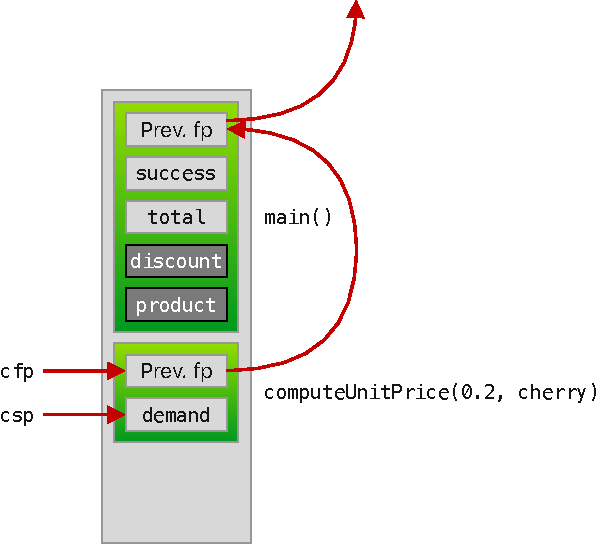
\includegraphics{Images/GCCC Stack.pdf}
	\end{center}
	\caption{A call stack containing two call frames in a variation of GCCC where no registers are available for storing parameters and local variables. The first call frame belongs to the initial procedure \texttt{main} which is called by the runtime, a dynamic linker, or the operating system and takes no parameters. Its call frame contains a \emph{previous frame pointer} capability that points to an unspecified location (possibly \texttt{null}) as well as two local variables \texttt{discount} and \texttt{price}. \texttt{main} invokes the 2-parameter \texttt{computeUnitPrice} procedure, binding the value \texttt{0.2} to the \texttt{discount} parameter and \texttt{cherry} to the \texttt{product} parameter. The latter procedure's call frame contains a \emph{previous frame pointer} capability that points to the location of the \emph{previous frame pointer} capability in the previous call frame, as well as a local variable \texttt{demand}. This call frame is at the top of the stack and so the \texttt{cfp} register's capability points to the \emph{previous frame pointer} capability in \texttt{computeUnitPrice}'s call frame. The \texttt{csp} register's capability always points to the last datum pushed on the stack, which is \texttt{demand} in this example. Note that the stack grows downward.}
	\label{fig:gcccstack}
\end{figure}

% TODO

\section{Abstract Locations}
% TODO

\section{Structured Jumps \& Branches}
% TODO

\section{Basic Abstractions over Assembly}
% TODO

\biblio{}
\onlyinsubfile{\glsaddall\printglossaries}
\end{document}
